El \textbf{Simple Network Management Protocol (SNMP)} es un protocolo de la capa de aplicación de la suite TCP/IP diseñado para la gestión y supervisión remota de dispositivos de red, tales como routers, switches, servidores, impresoras y otros equipos conectados. Su funcionamiento se basa en la interacción entre una estación de gestión (\textit{Manager}) y los dispositivos administrados (\textit{Agents}), permitiendo obtener información sobre el estado de la infraestructura, recopilar estadísticas, detectar fallos y modificar determinados parámetros de configuración.

Gracias a su simplicidad, bajo consumo de recursos e interoperabilidad entre dispositivos de distintos fabricantes, SNMP se consolidó como el estándar de facto para la administración de redes. Su utilización permite centralizar las tareas de monitorización y control, facilitando la supervisión de infraestructuras heterogéneas desde una única plataforma de gestión mediante consultas periódicas y notificaciones ante eventos relevantes.

\subsection{Historia y Evolución de SNMP}

Desde su aparición a finales de la década de 1980, SNMP ha evolucionado para responder a las necesidades crecientes de administración de redes. Aunque todas las versiones conservan el mismo modelo básico de funcionamiento, cada una incorporó mejoras destinadas a resolver limitaciones detectadas en versiones anteriores.

\subsubsection{SNMPv1}

Publicada en 1988, la primera versión de SNMP se convirtió rápidamente en el estándar dominante para la gestión de redes. Su diseño sencillo permitía una implementación eficiente y requería pocos recursos de procesamiento y ancho de banda.

SNMPv1 definió las operaciones fundamentales del protocolo, incluyendo \textit{GetRequest}, \textit{GetNextRequest}, \textit{SetRequest} y \textit{Trap}. Estas operaciones establecieron el modelo básico de comunicación que continúa siendo utilizado en las versiones actuales.

Sin embargo, presentaba limitaciones importantes. La autenticación se basaba únicamente en \textit{community strings} transmitidas en texto plano, mientras que el manejo de errores resultaba poco eficiente cuando una solicitud involucraba múltiples objetos de la MIB.

\subsubsection{SNMPv2 y SNMPv2c}

La segunda generación del protocolo surgió con el objetivo de mejorar la eficiencia operativa y el rendimiento de las tareas de gestión.

Entre sus principales aportes se encuentra la incorporación de la operación \textit{GetBulkRequest}, diseñada para recuperar grandes cantidades de información mediante una única transacción. Esta funcionalidad permite consultar tablas completas de la MIB con una cantidad significativamente menor de intercambios de mensajes.

Asimismo, se optimizó el tratamiento de errores y se incorporó la operación \textit{InformRequest}, que permite enviar notificaciones confirmadas entre estaciones de gestión.

Aunque se propusieron nuevos mecanismos de seguridad, la variante más difundida fue SNMPv2c, que continuó utilizando el esquema de autenticación basado en comunidades heredado de SNMPv1.

\subsubsection{SNMPv3}

La versión 3, publicada en 1998, mantuvo la compatibilidad funcional con SNMPv2, pero introdujo una arquitectura de seguridad robusta orientada a entornos productivos.

Su principal incorporación fue el \textit{User-based Security Model} (USM), encargado de proporcionar autenticación, integridad y confidencialidad para los mensajes intercambiados entre gestores y agentes. Adicionalmente, se introdujo el \textit{View-based Access Control Model} (VACM), que permite definir políticas detalladas de acceso a los objetos de la MIB.

Gracias a estas mejoras, SNMPv3 es actualmente la versión recomendada para infraestructuras donde la seguridad constituye un requisito fundamental.

\subsection{Arquitectura del Protocolo}

La arquitectura de SNMP está basada en tres componentes fundamentales: el \textit{Manager}, el \textit{Agent} y la \textit{Management Information Base} (MIB). Estos elementos trabajan conjuntamente para proporcionar una interfaz uniforme de administración independientemente del fabricante o del tipo de dispositivo gestionado.

\subsubsection{Manager}

El \textit{Manager} constituye el punto central de la administración de la red. Generalmente se implementa como una aplicación ejecutándose en un servidor o estación de gestión ubicada dentro de un Centro de Operaciones de Red (NOC).

Su función principal consiste en recopilar información proveniente de los dispositivos gestionados, analizar su estado operativo y traducir los requerimientos del administrador en comandos de gestión concretos. Para ello, el Manager inicia consultas periódicas hacia los agentes distribuidos en la infraestructura.

\subsubsection{Agent}

El \textit{Agent} es un proceso de software que se ejecuta dentro del dispositivo gestionado. Su responsabilidad consiste en recibir y procesar las solicitudes SNMP enviadas por el Manager.

Además de responder consultas, el Agent puede generar notificaciones asíncronas cuando ocurren eventos relevantes, como fallos de hardware, reinicios inesperados o cambios en el estado de una interfaz de red.

Internamente, el Agent actúa como intermediario entre la representación lógica de la información expuesta mediante SNMP y las estructuras de datos reales implementadas por el fabricante del dispositivo.

\subsubsection{Management Information Base (MIB)}

La \textit{Management Information Base} (MIB) es una representación lógica y jerárquica de los recursos administrables de un dispositivo. Contiene una colección de objetos que describen parámetros operativos, contadores estadísticos, estados y configuraciones.

Cada objeto se identifica mediante un \textit{Object Identifier} (OID), que permite localizarlo de forma única dentro de la estructura jerárquica de la MIB. Esta organización estandarizada facilita la interoperabilidad entre dispositivos de distintos fabricantes.

Los objetos suelen agruparse en categorías funcionales tales como \textit{system}, \textit{interfaces}, \textit{ip}, \textit{tcp} y \textit{udp}, entre otras.

\subsubsection{Interacción entre los Componentes}

El funcionamiento de SNMP se basa en la interacción constante entre estos tres elementos. El Manager envía solicitudes al Agent para consultar o modificar información. El Agent interpreta dichas solicitudes, accede a los objetos correspondientes dentro de la MIB y devuelve una respuesta con los datos solicitados o el resultado de la operación.

Esta separación entre gestión, procesamiento y representación de la información permite construir sistemas escalables y compatibles con infraestructuras heterogéneas.

\begin{figure}[H]
\centering
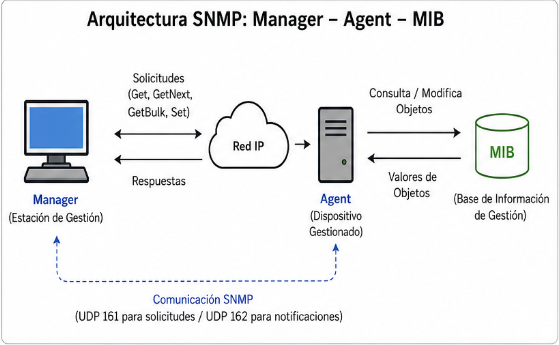
\includegraphics[width=0.5\textwidth]{img/snmp1.png}
\caption{Arquitectura básica de SNMP basada en la interacción entre Manager, Agent y MIB.}
\label{fig:snmp_arquitectura}
\end{figure}

\subsection{Transporte y Puertos Utilizados}

SNMP opera sobre la suite de protocolos TCP/IP y utiliza principalmente el protocolo \textit{User Datagram Protocol} (UDP) como mecanismo de transporte para el intercambio de mensajes entre los gestores y los agentes. Esta elección responde a la filosofía de diseño del protocolo, que prioriza la simplicidad, la eficiencia y el bajo consumo de recursos.

\subsubsection{Puertos UDP 161 y 162}

El estándar SNMP define dos puertos bien conocidos para diferenciar los distintos tipos de comunicación entre los componentes del sistema de gestión.

El puerto UDP 161 es utilizado por los agentes para recibir solicitudes provenientes de los gestores. A este puerto se envían operaciones como \textit{GetRequest}, \textit{GetNextRequest}, \textit{GetBulkRequest} y \textit{SetRequest}, que permiten consultar o modificar información contenida en la MIB del dispositivo.

Por otro lado, el puerto UDP 162 se reserva para el envío de notificaciones asíncronas. A través de este puerto, los agentes transmiten mensajes \textit{Trap} o \textit{InformRequest} destinados a alertar a los sistemas de gestión sobre eventos relevantes, fallos o cambios de estado ocurridos en el dispositivo.

\subsubsection{Razones para el Uso de UDP}

La utilización de UDP en lugar de protocolos orientados a conexión, como TCP, responde a varios criterios de diseño.

En primer lugar, UDP presenta una implementación sencilla y una sobrecarga mínima. Al no requerir establecimiento ni mantenimiento de conexiones, reduce el consumo de recursos tanto en los dispositivos gestionados como en la infraestructura de red.

Además, el modelo operativo de SNMP se basa principalmente en intercambios independientes de solicitud y respuesta. Cada consulta realizada por un Manager constituye una transacción individual, por lo que no resulta necesario mantener sesiones permanentes con los distintos agentes distribuidos en la red.

Otro aspecto importante es la capacidad de funcionamiento en escenarios de congestión o degradación de la red. Dado que la gestión suele ser especialmente necesaria durante situaciones de fallo, la baja sobrecarga introducida por UDP aumenta la probabilidad de que los mensajes de administración puedan llegar a destino incluso bajo condiciones adversas.

La ausencia de mecanismos de fiabilidad a nivel de transporte implica que la responsabilidad de detectar pérdidas y gestionar retransmisiones recae sobre la propia aplicación SNMP. Para ello, cada solicitud incorpora un identificador único que permite asociar las respuestas correspondientes y detectar posibles pérdidas de mensajes.

\subsection{Operaciones Fundamentales de SNMP}

La interacción entre gestores y agentes se realiza mediante un conjunto reducido de Unidades de Datos de Protocolo (PDU). Estas operaciones permiten consultar información, modificar configuraciones y recibir notificaciones sobre eventos relevantes dentro de la infraestructura administrada.

\subsubsection{Operaciones de Consulta}

Las operaciones de consulta permiten recuperar información almacenada en la MIB de un dispositivo.

\paragraph{GetRequest}

Es la operación básica de lectura. Permite al Manager solicitar el valor asociado a uno o varios objetos específicos identificados mediante sus correspondientes OID. El Agent procesa la solicitud y responde con una PDU \textit{Response} que contiene los valores requeridos.

\paragraph{GetNextRequest}

Esta operación permite obtener el objeto que sigue inmediatamente al OID especificado según el orden lexicográfico de la MIB. Su principal utilidad consiste en recorrer estructuras jerárquicas y tablas cuyos elementos no son conocidos previamente por el sistema de gestión.

\paragraph{GetBulkRequest}

Introducida en SNMPv2, esta operación fue diseñada para optimizar la recuperación masiva de información. Permite obtener múltiples objetos mediante una única solicitud, reduciendo significativamente la cantidad de mensajes intercambiados y mejorando la eficiencia en la consulta de tablas extensas.

\subsubsection{Operaciones de Modificación}

\paragraph{SetRequest}

La operación \textit{SetRequest} permite modificar el valor de uno o varios objetos administrados dentro de un dispositivo. Gracias a esta funcionalidad, un sistema de gestión puede alterar determinados parámetros operativos de forma remota.

Una característica importante de esta operación es su comportamiento atómico. Si una solicitud involucra múltiples modificaciones y alguna de ellas no puede completarse correctamente, el agente cancela la totalidad de la operación para preservar la consistencia de la configuración.

\subsubsection{Operaciones de Notificación}

Las operaciones de notificación permiten que un dispositivo informe eventos relevantes sin necesidad de esperar una consulta previa del sistema de gestión.

\paragraph{Trap}

Un \textit{Trap} es una notificación asíncrona enviada por el Agent cuando ocurre un evento significativo, como la caída de una interfaz, un reinicio inesperado o un intento fallido de autenticación. Este mecanismo permite reducir la necesidad de realizar consultas constantes sobre el estado del dispositivo.

Sin embargo, debido al uso de UDP, los mensajes \textit{Trap} no requieren confirmación por parte del receptor. En consecuencia, existe la posibilidad de que una notificación se pierda durante la transmisión.

\paragraph{InformRequest}

La operación \textit{InformRequest}, incorporada en SNMPv2, extiende el concepto de notificación agregando un mecanismo de confirmación. Una vez recibido el mensaje, el destinatario debe responder mediante una PDU \textit{Response}, garantizando que la información fue efectivamente entregada.

\begin{figure}[H]
\centering
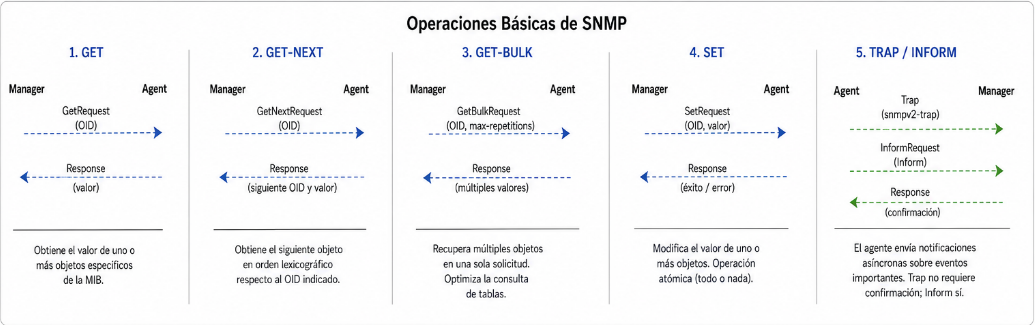
\includegraphics[width=1\textwidth]{img/snmp2.png}
\caption{Principales operaciones utilizadas por el protocolo SNMP para consulta, modificación y notificación.}
\label{fig}
\end{figure}

\subsection{Modelo de Comunicación: Polling y Notificaciones}

El funcionamiento de SNMP combina dos mecanismos complementarios de comunicación: el modelo tradicional de \textit{polling}, basado en solicitudes periódicas realizadas por el sistema de gestión, y las notificaciones asíncronas generadas por los dispositivos cuando ocurre un evento relevante.

\subsubsection{Modelo de Polling}

El \textit{polling} constituye el mecanismo predominante en la mayoría de las implementaciones SNMP. En este modelo, el Manager inicia la comunicación enviando consultas periódicas a los agentes para conocer el estado de los dispositivos y recopilar métricas operativas.

La frecuencia de estas consultas es definida por el administrador, permitiendo controlar el volumen de tráfico de gestión generado en la red. Este enfoque proporciona una visión continua del estado de la infraestructura y facilita la construcción de series históricas para el análisis de rendimiento.

No obstante, cuando el número de dispositivos es elevado o los intervalos de consulta son demasiado cortos, el tráfico generado por el proceso de monitorización puede aumentar considerablemente.

\subsubsection{Notificaciones Asíncronas}

Las notificaciones asíncronas permiten que el Agent tome la iniciativa de comunicación cuando detecta un evento significativo. En lugar de esperar una consulta periódica, el dispositivo informa inmediatamente la ocurrencia del suceso mediante un mensaje \textit{Trap} o \textit{InformRequest}.

Este mecanismo resulta especialmente eficiente para la detección temprana de fallos, ya que elimina la necesidad de realizar consultas constantes sobre eventos poco frecuentes.

Sin embargo, los mensajes \textit{Trap} presentan una limitación importante: al no requerir confirmación, pueden perderse sin que el Manager tenga conocimiento de ello. Para situaciones donde la confiabilidad resulta crítica, es posible utilizar \textit{InformRequest}, que incorpora un mecanismo explícito de confirmación de recepción.

En la práctica, los sistemas modernos de monitorización combinan ambos enfoques. El \textit{polling} proporciona una supervisión continua de métricas y estados operativos, mientras que las notificaciones permiten reaccionar rápidamente ante eventos críticos sin generar tráfico innecesario.

